\documentclass[11pt,UTF8]{ctexart}


\usepackage[margin=2cm,a4paper]{geometry}
%\usepackage[left=0.75in,top=0.6in,right=0.75in,bottom=1.0in,a4paper]{geometry}

\setmainfont{Caladea}
%% 也可以選用其它字庫:
% \setCJKmainfont[%
%   ItalicFont=AR PL KaitiM GB,
%   BoldFont=Noto Sans CJK SC,
% ]{Noto Serif CJK SC}
% \setCJKsansfont{Noto Sans CJK SC}
% \renewcommand{\kaishu}{\CJKfontspec{AR PL KaitiM GB}}

% 繁體中文
\setCJKmainfont[Path=fonts/ ]{NotoSansTC-Medium.otf}

\usepackage{minted}
\usepackage[breaklinks]{hyperref}

% Picture
% 導言區的此三行無變化
\usepackage{graphicx}
\usepackage{float} 
\usepackage{subfigure}
% 以下是新增的自定義格式更改
\usepackage[]{caption2} %新增調用的宏包
\renewcommand{\figurename}{Fig.} %重定義編號前綴詞
\renewcommand{\captionlabeldelim}{.~} %重定義分隔符
 %\roman 是羅馬數字編號,\alph是默認的字母編號,\arabic是阿拉伯數字編號,可按需替換下一行的相應位置
\renewcommand{\thesubfigure}{(\roman{subfigure})}%此外,還可設置圖編號顯示格式,加括號或者不加括號
\makeatletter \renewcommand{\@thesubfigure}{\thesubfigure \space}%子圖編號與名稱的間隔設置
\renewcommand{\p@subfigure}{} \makeatother

% Math
\usepackage {mathtools}
\usepackage{amssymb}

% Code
\usepackage{listings}
\usepackage{xcolor}
\lstset{
    % backgroundcolor=\color{red!50!green!50!blue!50},
    % 程式碼塊背景色為淺灰色
    rulesepcolor= \color{gray}, % 程式碼塊邊框顏色
    breaklines=true,  % 程式碼過長則換行
    numbers=left, % 行號在左側顯示
    numberstyle= \small,% 行號字型
    % eywordstyle= \color{red,% 關鍵字顏色
    commentstyle=\color{gray}, % 註釋顏色
    frame=shadowbox % 用方框框住程式碼塊
    }

\usepackage{hyperref}

\title{計算機視覺作業}
\author{干皓丞,2101212850, 信息工程學院}

\begin{document}
\maketitle


\section{作業目標與章節摘要}

在 GitHub 或者任意頁面下載超分算法,獲得結果試著訓練 1 ~ 2 個 Epoch,並給出分析結果,原始程式碼在名為 kancheng/kan-cs-report-in-2021 的 Github 專案下,可以在 CV/super-resolution/code 下找到。

\begin{figure}[H]
\centering 

\includegraphics[width=0.9\textwidth]{t1.png} 
\caption{作業目標}
\label{Test}
\end{figure}

\section{Practice CNN}

在此將上次課程的範例與 MNIST 做一個練習,可以在專案目錄 CV/super-resolution/code 下找到名為 cnn-each-init-method.ipynb 的檔案,該剛檔案對範例的 LeNet、AlexNet、VGG、GoogLeNet、ResNet、ShuffleNet、Res2Net、DenseNet等,CNN 程式碼進行複習,對應後面的超分算法 SRCNN 會比較有感覺。

\section{Pytorch SRCNN}

Pytorch SRCNN 分為兩類,一個為 Pytorch 撰寫的 *.py 檔案,在 CV/super-resolution/code 下的 pytorch-srcnn,可以直接用指令執行,同時額外寫一個版本為 *.ipynb,方便進行呈現,檔名為  pytorch-srcnn-demo.ipynb。該專案測試訓練資料的放置於 kancheng/training-data 下的相同名稱的目錄。兩個版本的差異在於目錄配置不同。其兩者的目錄檔案目錄配置如下。input 目錄為放置訓練測試資料,outputs 為放置輸出結果,而 *.py 版本則是有一個名為 src 的目錄,當中分別為代表 SRCNN 的 srcnn.py、訓練的 train.py 與測試的 test.py,而 *.ipynb 版本則為單純的呈現,為了證明可執行 Epoch 值在 pytorch-srcnn-demo.ipynb 中設定為 ,而 *.py 則是有 Epoch 值設定為 100,後續呈現程式碼的部分為 *.ipynb 的版本,而測試結果為 *.py 的版本。

下為 Pytorch SRCNN 的 *.py 與 *.ipynb 版本目錄配置。

\begin{figure}[H]
\centering 
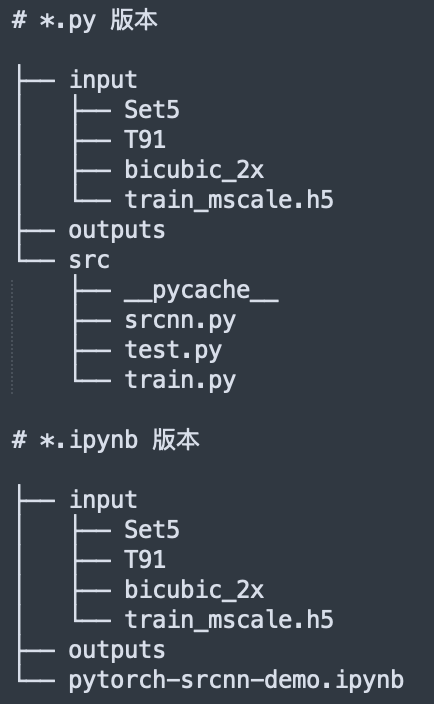
\includegraphics[width=0.30\textwidth]{s1.png} 
\caption{Pytorch SRCNN 目錄配置}
\label{Test}
\end{figure}


Pytorch SRCNN 的程式碼如下所示。

	\begin{lstlisting}[language={python}]
import torch.nn as nn
import torch.nn.functional as F
class SRCNN(nn.Module):
    def __init__(self):
        super(SRCNN, self).__init__()
        self.conv1 = nn.Conv2d(1, 64, kernel_size=9, padding=2, padding_mode='replicate') 
        # padding mode same as original Caffe code
        self.conv2 = nn.Conv2d(64, 32, kernel_size=1, padding=2, padding_mode='replicate')
        self.conv3 = nn.Conv2d(32, 1, kernel_size=5, padding=2, padding_mode='replicate')
    def forward(self, x):
        x = F.relu(self.conv1(x))
        x = F.relu(self.conv2(x))
        x = self.conv3(x)
        return x
import torch
import matplotlib
import matplotlib.pyplot as plt
import time
import h5py
# import srcnn
import torch.optim as optim
import torch.nn as nn
import numpy as np
import math
from torch.utils.data import DataLoader, Dataset
from tqdm import tqdm
from sklearn.model_selection import train_test_split
from torchvision.utils import save_image
matplotlib.style.use('ggplot')

# learning parameters
batch_size = 64 # batch size, reduce if facing OOM error
epochs = 2
# epochs = 100
# number of epochs to train the SRCNN model for
lr = 0.001 # the learning rate
device = 'cuda' if torch.cuda.is_available() else 'cpu'

# input image dimensions
img_rows, img_cols = 33, 33
out_rows, out_cols = 33, 33

# file = h5py.File('../input/train_mscale.h5')
file = h5py.File('./input/train_mscale.h5')
# `in_train` has shape (21884, 33, 33, 1) which corresponds to
# 21884 image patches of 33 pixels height & width and 1 color channel
in_train = file['data'][:] # the training data
out_train = file['label'][:] # the training labels
file.close()
# change the values to float32
in_train = in_train.astype('float32')
out_train = out_train.astype('float32')

(x_train, x_val, y_train, y_val) = train_test_split(in_train, out_train, test_size=0.25)
print('Training samples: ', x_train.shape[0])
print('Validation samples: ', x_val.shape[0])

# the dataset module
class SRCNNDataset(Dataset):
    def __init__(self, image_data, labels):
        self.image_data = image_data
        self.labels = labels
    def __len__(self):
        return (len(self.image_data))
    def __getitem__(self, index):
        image = self.image_data[index]
        label = self.labels[index]
        return (
            torch.tensor(image, dtype=torch.float),
            torch.tensor(label, dtype=torch.float)
        )


# train and validation data
train_data = SRCNNDataset(x_train, y_train)
val_data = SRCNNDataset(x_val, y_val)
# train and validation loaders
train_loader = DataLoader(train_data, batch_size=batch_size)
val_loader = DataLoader(val_data, batch_size=batch_size)

# initialize the model
print('Computation device: ', device)
model = SRCNN().to(device)
print(model)

# optimizer
optimizer = optim.Adam(model.parameters(), lr=lr)
# loss function 
criterion = nn.MSELoss()

def psnr(label, outputs, max_val=1.):
    """
    Compute Peak Signal to Noise Ratio (the higher the better).
    PSNR = 20 * log10(MAXp) - 10 * log10(MSE).
    https://en.wikipedia.org/wiki/Peak_signal-to-noise_ratio#Definition
    First we need to convert torch tensors to NumPy operable.
    """
    label = label.cpu().detach().numpy()
    outputs = outputs.cpu().detach().numpy()
    img_diff = outputs - label
    rmse = math.sqrt(np.mean((img_diff) ** 2))
    if rmse == 0:
        return 100
    else:
        PSNR = 20 * math.log10(max_val / rmse)
        return PSNR



def train(model, dataloader):
    model.train()
    running_loss = 0.0
    running_psnr = 0.0
    for bi, data in tqdm(enumerate(dataloader), total=int(len(train_data)/dataloader.batch_size)):
        image_data = data[0].to(device)
        label = data[1].to(device)
        
        # zero grad the optimizer
        optimizer.zero_grad()
        outputs = model(image_data)
        loss = criterion(outputs, label)
        # backpropagation
        loss.backward()
        # update the parameters
        optimizer.step()
        # add loss of each item (total items in a batch = batch size)
        running_loss += loss.item()
        # calculate batch psnr (once every `batch_size` iterations)
        batch_psnr =  psnr(label, outputs)
        running_psnr += batch_psnr
    final_loss = running_loss/len(dataloader.dataset)
    final_psnr = running_psnr/int(len(train_data)/dataloader.batch_size)
    return final_loss, final_psnr


def validate(model, dataloader, epoch):
    model.eval()
    running_loss = 0.0
    running_psnr = 0.0
    with torch.no_grad():
        for bi, data in tqdm(enumerate(dataloader), total=int(len(val_data)/dataloader.batch_size)):
            image_data = data[0].to(device)
            label = data[1].to(device)
            
            outputs = model(image_data)
            loss = criterion(outputs, label)
            # add loss of each item (total items in a batch = batch size) 
            running_loss += loss.item()
            # calculate batch psnr (once every `batch_size` iterations)
            batch_psnr = psnr(label, outputs)
            running_psnr += batch_psnr
        outputs = outputs.cpu()
        save_image(outputs, f"./outputs/val_sr{epoch}.png")
    final_loss = running_loss/len(dataloader.dataset)
    final_psnr = running_psnr/int(len(val_data)/dataloader.batch_size)
    return final_loss, final_psnr


train_loss, val_loss = [], []
train_psnr, val_psnr = [], []
start = time.time()
for epoch in range(epochs):
    print(f"Epoch {epoch + 1} of {epochs}")
    train_epoch_loss, train_epoch_psnr = train(model, train_loader)
    val_epoch_loss, val_epoch_psnr = validate(model, val_loader, epoch)
    print(f"Train PSNR: {train_epoch_psnr:.3f}")
    print(f"Val PSNR: {val_epoch_psnr:.3f}")
    train_loss.append(train_epoch_loss)
    train_psnr.append(train_epoch_psnr)
    val_loss.append(val_epoch_loss)
    val_psnr.append(val_epoch_psnr)
end = time.time()
print(f"Finished training in: {((end-start)/60):.3f} minutes")


# loss plots
plt.figure(figsize=(10, 7))
plt.plot(train_loss, color='orange', label='train loss')
plt.plot(val_loss, color='red', label='validataion loss')
plt.xlabel('Epochs')
plt.ylabel('Loss')
plt.legend()
plt.savefig('./outputs/loss.png')
plt.show()
# psnr plots
plt.figure(figsize=(10, 7))
plt.plot(train_psnr, color='green', label='train PSNR dB')
plt.plot(val_psnr, color='blue', label='validataion PSNR dB')
plt.xlabel('Epochs')
plt.ylabel('PSNR (dB)')
plt.legend()
plt.savefig('./outputs/psnr.png')
plt.show()
# save the model to disk
print('Saving model...')
torch.save(model.state_dict(), './outputs/model.pth')
	\end{lstlisting}

從測試結果中可以看到 Epochs 設定為 100 時,Train Loss 很快的下降,同時 PSNR 也平穩,同時也可以從訓練後的結果中可看到相對原本清晰的結果。若 Epochs 設定更高時,或許可以有更好的結果。而訓練與測試過程中的指令輸出結果則被記錄在專案目錄下的 command-line-record.md 檔案。

\begin{figure}[H]
\centering  %圖片全局居中
\subfigure[Train Loss]{
\label{Fig.sub.1}
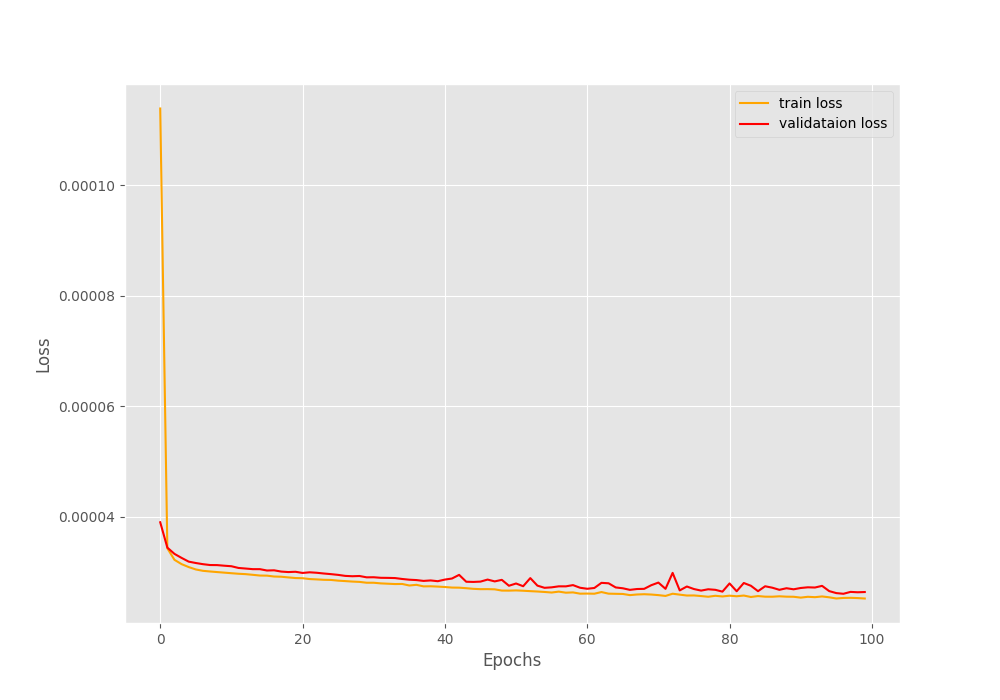
\includegraphics[width=0.45\textwidth]{s2.png}}
\subfigure[PSNR]{
\label{Fig.sub.2}
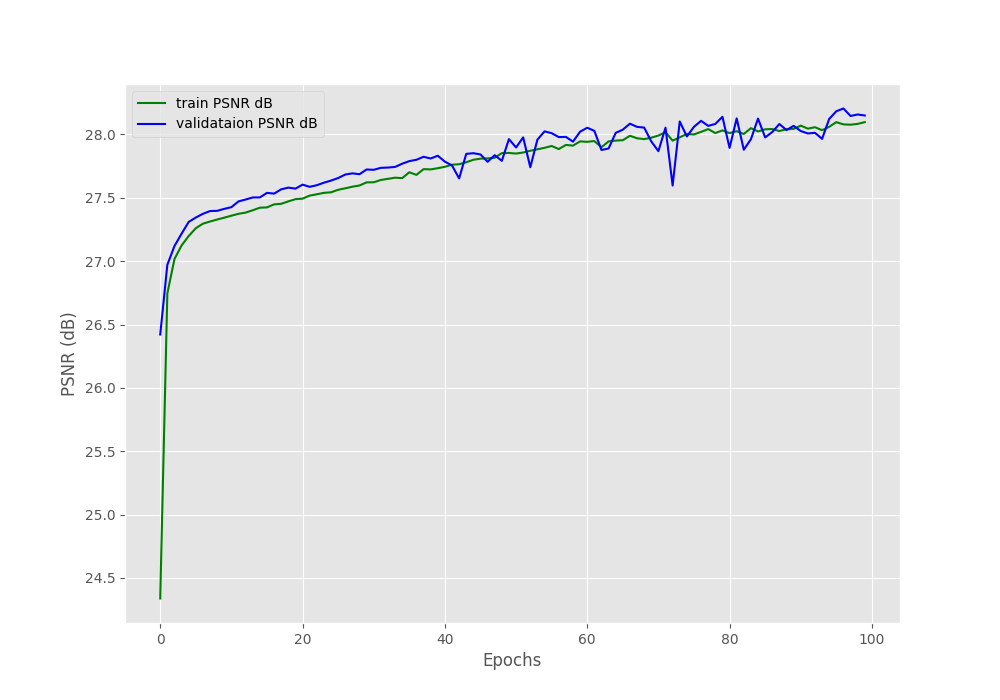
\includegraphics[width=0.45\textwidth]{s3.png}}
\caption{訓練}
\label{Fig.main}
\end{figure}


\begin{figure}[H]
\centering 
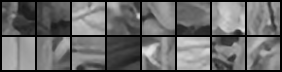
\includegraphics[width=0.80\textwidth]{s4.png} 
\caption{Pytorch SRCNN 訓練過程}
\label{Test}
\end{figure}


\begin{figure}[H]
\centering  %圖片全局居中
\subfigure[Output]{
\label{Fig.sub.1}

\includegraphics[width=0.45\textwidth]{s5.png}}
\subfigure[Test]{
\label{Fig.sub.2}

\includegraphics[width=0.45\textwidth]{s6.png}}
\caption{輸出測試結果}
\label{Fig.main}
\end{figure}

\begin{center}
\begin{tabular}{ccc}
\hline
Epoch & Train PSNR & Val PSNR \\
\hline
10 & 27.343 & 27.413 \\
20 & 27.489 & 27.572 \\
30 & 27.622 & 27.723 \\
40 & 27.734 & 27.832 \\
50 & 27.854 & 27.963 \\
60 & 27.945 & 28.022 \\
70 & 27.974 & 27.945 \\
80 & 28.032 & 28.139 \\
90 & 28.043 & 28.068 \\ 
100 & 28.097 & 28.149 \\
\hline
\end{tabular}
\end{center}
                                                                                                                  

% \newpage
\newpage

\section{Tensorflow SRCNN}

Tensorflow SRCNN 在此為單純的 *.py 檔案,在 CV/super-resolution/code 下的 tensorflow-srcnn,可以直接用指令執行。該專案測試訓練資料的放置於 kancheng/training-data 下的相同名稱的目錄,而訓練與測試過程中的指令輸出結果則被記錄在專案目錄下的 command-line-record.md 檔案。當中需要注意的是 Mac 使用者很有可能會在測試時遇到 .DS\_store 的問題,建議可以使用指令進行暫時性處理。另外若想要放置自己測試的資料必須放在該專案目錄下的 Test 目錄,同時要符合該專案的結構。


\begin{verbatim}
$ sudo find /Users/[ Path ]/ -name ".DS_Store" -depth -exec rm {} \;
\end{verbatim}

同時在測試與訓練過程需要注意的地方在於,參與預設的細節另外,其參數範例如下所示。

\begin{verbatim}
# Training SRCNN
# Quick training
$ python main.py

# Example usage
$ python main.py --use_pretrained=False \
    --epoch=1000 \
    --scale=4 \
    
# Testing SRCNN
# Quick testing
$ python main.py --is_training=False \
    --use_pretrained=True

# Example usage
$ python main.py --is_training=False \
    --use_pretrained=True \
    --test_dataset=YOUR_DATASET \
    --scale=4

# 若想自行加入資料
#  Test 为測試資料目录名稱
$ python main.py --is_training=False \
    --use_pretrained=True \
    --test_dataset=Test \
    --scale=4
\end{verbatim}


\begin{figure}[H]
\centering 
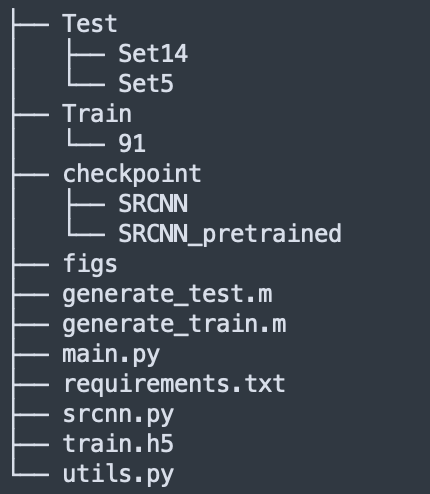
\includegraphics[width=0.30\textwidth]{tf1.png} 
\caption{Tensorflow SRCNN 目錄配置}
\label{Test}
\end{figure}

main.py 程式碼如下所示。

	\begin{lstlisting}[language={python}]
# import tensorflow as tf
import tensorflow
import tensorflow.compat.v1 as tf
from srcnn import SRCNN


# flags = tf.app.flags
flags = tf.compat.v1.app.flags
flags.DEFINE_integer('epoch', 10000, 'Number of epoch')
flags.DEFINE_integer('batch_size', 128, 'The size of batch images')
flags.DEFINE_integer('image_size', 33, 'The size of sub-image')
flags.DEFINE_integer('label_size', 21, 'The size of label')

flags.DEFINE_integer('scale', 3, 'The up-scale value for training and testing')

flags.DEFINE_float('learning_rate', 1e-4, 'The learning rate of gradient descent algorithm')
flags.DEFINE_float('beta1', 0.9, 'The momentum value of gradient descent algorithm')

flags.DEFINE_string('valid_dataset', 'Set5', 'The name of training dataset')
flags.DEFINE_string('test_dataset_path', 'Test', 'The path of test dataset')
flags.DEFINE_string('test_dataset', 'Set5', 'The name of testing dataset')

flags.DEFINE_string('checkpoint_path', 'checkpoint', 'The path of checkpoint directory')
flags.DEFINE_boolean('use_pretrained', False, 'True for use pre-trained model, False for train on your own')
flags.DEFINE_string('result_dir', 'result', 'The path to save result images')
flags.DEFINE_boolean('is_training', True, 'True for training, False for testing')

FLAGS = flags.FLAGS


def main(_):
    with tf.Session() as sess:
        srcnn = SRCNN(sess, FLAGS)

        if FLAGS.is_training == True:
            srcnn.train(FLAGS)

        elif FLAGS.is_training == False:
            srcnn.test(FLAGS)

        else:
            print('[*] Please give correct [is_training] value ')

if __name__ == '__main__':
    tf.app.run()
	\end{lstlisting}

srcnn.py 程式碼如下所示。

	\begin{lstlisting}[language={python}]
import tensorflow as tf
import numpy as np

import os
import time
from tqdm import tqdm

from utils import *


class SRCNN(object):
    def __init__(self, sess, config):
        self.sess = sess

        # The size of training sub-images is 33
        # All the convolutional layers have no padding (fsub-f1-f2-f3+3) = (33-5-9-1+3) = 21
        self.image_size = [None, None, None, 1]
        self.label_size = [None, None, None, 1]

        self.build_model()
    

    def build_model(self):
        self.images = tf.placeholder(tf.float32, self.image_size, name='images')
        self.labels = tf.placeholder(tf.float32, self.label_size, name='labels')

        self.weights = {
            'w1': tf.Variable(tf.random_normal([9, 9, 1, 64], stddev=0.001), name='w1'),
            'w2': tf.Variable(tf.random_normal([1, 1, 64, 32], stddev=0.001), name='w2'),
            'w3': tf.Variable(tf.random_normal([5, 5, 32, 1], stddev=0.001), name='w3')
        }
        self.biases = {
            'b1': tf.Variable(tf.zeros([64]), name='b1'),
            'b2': tf.Variable(tf.zeros([32]), name='b2'),
            'b3': tf.Variable(tf.zeros([1]), name='b3')
        }

        self.forward = self.model()

        # Loss Function : Mean Square Error
        self.loss = tf.reduce_mean(tf.square(tf.subtract(self.labels, self.forward)))

        # Clip output
        self.result = tf.clip_by_value(self.forward, clip_value_min=0., clip_value_max=1.)

        self.saver = tf.train.Saver()


    # Input  : (33 x 33 x 1)
    # Layer1 : (9 x 9 x 1 x 64)
    # Layer2 : (1 x 1 x 64 x 32)
    # Layer3 : (5 x 5 x 32 x 1)
    # Output : (21 x 21 x 1)
    def model(self):
        conv1 = tf.nn.relu(tf.nn.bias_add(tf.nn.conv2d(self.images, self.weights['w1'], strides=[1,1,1,1], padding='VALID'), self.biases['b1']))

        conv2 = tf.nn.relu(tf.nn.bias_add(tf.nn.conv2d(conv1, self.weights['w2'], strides=[1,1,1,1], padding='VALID'), self.biases['b2']))
       
        output = tf.nn.bias_add(tf.nn.conv2d(conv2, self.weights['w3'], strides=[1,1,1,1], padding='VALID'), self.biases['b3'])
    
        return output


    def train(self, config):
        print('[*] SRCNN training will be started ! ')

        if not exist_train_data():
            print('[!] No train data ready .. Please generate train data first with Matlab')
            return
        else:
            train_images, train_labels = load_train_data()
            print('[*] Successfully load train data ! ')
       
        valid_images, valid_labels = prepare_data(config, is_valid=True)

        # Adam optimizer with the standard backpropagation
        # The learning rate is 1e-4 for the first two layers, and 1e-5 for the last layer
        # beta1 is 0.9 in paper
        var_list1 = [self.weights['w1'], self.weights['w2'], self.biases['b1'], self.biases['b2']]
        var_list2 = [self.weights['w3'], self.biases['b3']]
        opt1 = tf.train.AdamOptimizer(config.learning_rate, beta1=config.beta1)
        opt2 = tf.train.AdamOptimizer(config.learning_rate * 0.1, beta1=config.beta1)
        grads = tf.gradients(self.loss, var_list1 + var_list2)
        grads1 = grads[:len(var_list1)]
        grads2 = grads[len(var_list1):]
        train_op1 = opt1.apply_gradients(zip(grads1, var_list1))
        train_op2 = opt2.apply_gradients(zip(grads2, var_list2))
        self.train_op = tf.group(train_op1, train_op2)

        #self.train_op = tf.train.AdamOptimizer(self.learning_rate).minimize(self.loss)

        # Initialize TensorFlow variables
        init = tf.global_variables_initializer()
        self.sess.run(init)

        # Load checkpoint
        self.load(config)

        start_time = time.time()
        bicubic_psnr = []
        print('[*] Start training ... Please be patient !')
        for i in tqdm(range(config.epoch), desc='[*] Keep going ! ', leave=True):
            loss = 0
            batch_idxs = len(train_images) // config.batch_size
            
            for idx in range(batch_idxs):
                batch_images = train_images[idx*config.batch_size : (idx+1)*config.batch_size]
                batch_labels = train_labels[idx*config.batch_size : (idx+1)*config.batch_size]
            
                _, err = self.sess.run([self.train_op, self.loss], feed_dict={self.images: batch_images, self.labels: batch_labels})
                loss += err

            valid_psnr = []
            for idx in range(len(valid_images)):
                h, w, _ = valid_images[idx].shape
                valid_input_y = valid_images[idx][:, :, 0]
                valid_label_y = valid_labels[idx][:, :, 0]

                valid_input_y = valid_input_y.reshape([1, h, w, 1])
                valid_label_y = valid_label_y.reshape([1, h, w, 1])

                result = self.sess.run(self.result, feed_dict={self.images: valid_input_y, self.labels: valid_label_y})
                
                valid_label_y = crop_border(valid_label_y[0])

                if i == 0:
                        bicubic_psnr.append(psnr(valid_label_y, crop_border(valid_input_y[0])))
                valid_psnr.append(psnr(valid_label_y, result[0]))
                
            print('[*] Epoch: [{:d}], psnr: [bicubic: {:.2f}, srcnn: {:.2f}], loss: [{:.8f}]'.format(i+1, np.mean(bicubic_psnr), np.mean(valid_psnr), loss/batch_idxs))
            
            # Save model for every 50 epoch
            if (i+1) % 50 == 0:
                self.save(i+1, config)
        print('[*] Training done ! Congrats :) ')
    

    def test(self, config):
        print('[*] SRCNN testing will be started ! ')
        t = time.strftime('%Y-%m-%d-%H%M%S', time.localtime(time.time()))

        test_images, test_labels = prepare_data(config, is_valid=False)

        init = tf.global_variables_initializer()

        results = []
        bicubic_psnr = []
        test_psnr = []
        print('[*] Start testing !')
        
        self.sess.run(init)
        
        self.load(config)

        for idx in tqdm(range(len(test_images))):
            h, w, _ = test_images[idx].shape
            test_input_y = test_images[idx][:, :, 0]
            test_label_y = test_labels[idx][:, :, 0]

            test_input_cbcr = test_images[idx][:, :, 1:3]
            test_label_cbcr = test_labels[idx][:, :, 1:3]

            test_input_y = test_input_y.reshape([1, h, w, 1])
            test_label_y = test_label_y.reshape([1, h, w, 1])

            test_input_cbcr = test_input_cbcr.reshape([1, h, w, 2])
            test_label_cbcr = test_label_cbcr.reshape([1, h, w, 2])

            result = self.sess.run(self.result, feed_dict={self.images: test_input_y, self.labels: test_label_y})
                
            test_input_y = crop_border(test_input_y[0])
            test_label_y = crop_border(test_label_y[0])

            test_input_cbcr = crop_border(test_input_cbcr[0])
            test_label_cbcr = crop_border(test_label_cbcr[0])

            bicubic_psnr.append(psnr(test_label_y, test_input_y))
            test_psnr.append(psnr(test_label_y, result[0]))

            gt = concat_ycrcb(test_label_y, test_label_cbcr)
            bicubic = concat_ycrcb(test_input_y, test_input_cbcr)
            result = concat_ycrcb(result[0], test_input_cbcr)
            
            path = os.path.join(os.getcwd(), config.result_dir)
            path = os.path.join(path, t)
            if not os.path.exists(path):
                os.makedirs(path)

            save_result(path, gt, bicubic, result, idx)
            
        print('[*] PSNR of ground truth and bicubic : {:.2f}'.format(np.mean(bicubic_psnr)))
        print('[*] PSNR of ground truth and SRCNN   : {:.2f}'.format(np.mean(test_psnr)))

        
    def save(self, epoch, config):
        model_name = 'srcnn'
        model_dir = 'SRCNN'
        path = os.path.join(config.checkpoint_path, model_dir)
        if not os.path.exists(path):
            os.makedirs(path)
        
        self.saver.save(self.sess, os.path.join(path, model_name), global_step=epoch)
        print('[*] Save checkpoint at {:d} epoch'.format(epoch))


    def load(self, config):
        if config.use_pretrained:
            model_dir = 'SRCNN_pretrained'
        else:
            model_dir = 'SRCNN'
        path = os.path.join(config.checkpoint_path, model_dir)
        ckpt_path = tf.train.latest_checkpoint(path)
        if ckpt_path:
            self.saver.restore(self.sess, ckpt_path)
            print('[*] Load checkpoint: {}'.format(ckpt_path))
        else:
            print('[*] No checkpoint to load ... ')
        
	\end{lstlisting}
	
utils.py 程式碼如下所示。

	\begin{lstlisting}[language={python}]
# import tensorflow as tf
import tensorflow
import tensorflow.compat.v1 as tf
import numpy as np
import math

from PIL import Image

from tqdm import tqdm

import os
import h5py

# FLAGS = tf.app.flags.FLAGS
FLAGS = tf.compat.v1.app.flags.FLAGS



# Read image
def imread(fname):
    return Image.open(fname)


# Save image
def imsave(image, path, fname):
    image = image * 255.
    
    image = Image.fromarray(image.astype('uint8'), mode='YCbCr')
    image = image.convert('RGB')
    
    return image.save(os.path.join(path, fname))


# Save ground truth image, bicubic interpolated image and srcnn image
def save_result(path, gt, bicubic, srcnn, i):
    imsave(gt, path, str(i)+ '_gt.png')
    imsave(bicubic, path, str(i) + '_bicubic.png')
    imsave(srcnn, path, str(i) + '_srcnn.png')


# Load sub-images of the dataset
def load_train_data():
    with h5py.File('train.h5', 'r') as f:
        images = np.array(f.get('data'))
        labels = np.array(f.get('label'))
    return images, labels


# Return true if the h5 sub-images file is exists
def exist_train_data():
    return os.path.exists('train.h5')


def prepare_data(config, is_valid=False):
    if is_valid:
        dataset = config.valid_dataset
        path = os.path.join(config.test_dataset_path, dataset)
    else:
        dataset = config.test_dataset
        path = os.path.join(config.test_dataset_path, dataset)

    dir_path = os.path.join(os.getcwd(), path)
    path_gt = os.path.join(dir_path, 'gt')
    path_lr = os.path.join(dir_path, 'bicubic_{:d}x'.format(config.scale))

    # fnames = ['baby_GT.bmp, bird_GT.bmp, ...']
    fnames = os.listdir(path_gt)
    
    inputs = []
    labels = []

    count = 0
    for fname in tqdm(fnames, desc='[*] Generating dataset ... '):
        count += 1
        
        _input = imread(os.path.join(path_lr, fname))
        _label = imread(os.path.join(path_gt, fname))
    
        _input = np.array(_input)
        _label = np.array(_label)
        
        inputs.append(_input / 255.)
        labels.append(_label / 255.)

    if is_valid:
        print('[*] Successfully prepared {:d} valid images !'.format(count))
    else:
        print('[*] Successfully prepared {:d} test images !'.format(count))
        
    return inputs, labels


# Concatenate Y and CrCb channel
def concat_ycrcb(y, crcb):
    return np.concatenate((y, crcb), axis=2)


# Crop border of the image
def crop_border(image):
    padding = int((5+9+1-3)/2)
    if image.ndim == 3:
        h, w, _ = image.shape
    else:
        h, w = image.shape

    return image[padding:h-padding, padding:w-padding]


# Compute Peak Signal to Noise Ratio
# PSNR = 20 * log (MAXi / root(MSE))
def psnr(label, image, max_val=1.):
    h, w, _ = label.shape

    diff = image - label
    rmse = math.sqrt(np.mean(diff ** 2))
    if rmse == 0:
        return 100
    else:
        return 20 * math.log10(max_val / rmse)
	\end{lstlisting}

下圖為測試結果與指令輸出整理。
	
\begin{figure}[H]
\centering  %圖片全局居中
\subfigure[Bicubic]{
\label{Fig.sub.1}
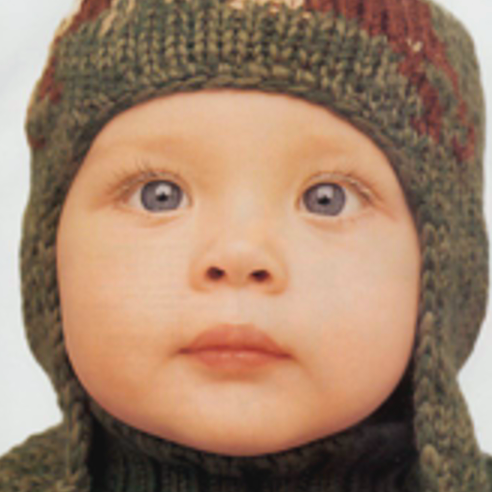
\includegraphics[width=0.3\textwidth]{tf2.png}}
\subfigure[GT]{
\label{Fig.sub.2}
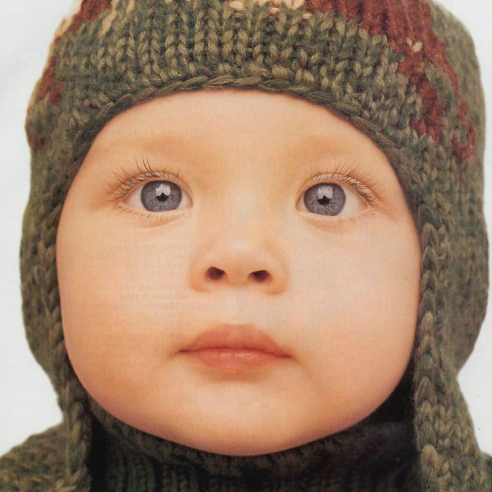
\includegraphics[width=0.3\textwidth]{tf3.png}}
\subfigure[SRCNN]{
\label{Fig.sub.3}
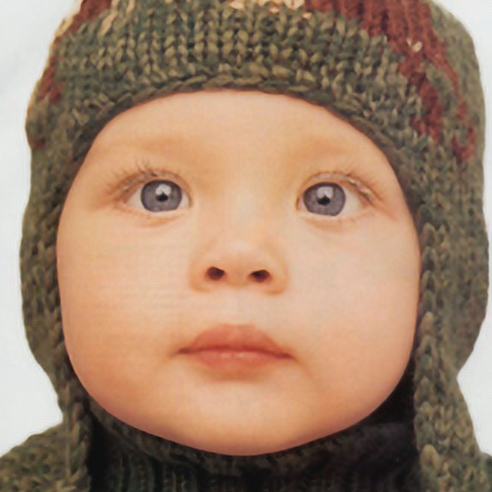
\includegraphics[width=0.3\textwidth]{tf4.png}}
\caption{測試結果}
\label{Fig.main}
\end{figure}

\begin{center}
\begin{tabular}{cccc}
\hline
Epoch & PSNR-Bicubic & PSNR-SRCNN & Loss  \\
\hline
 10 & 28.39 & 28.21 & 0.00225721 \\
 20 & 28.39 & 28.49 & 0.00206320 \\
 30 & 28.39 & 28.78 & 0.00183421 \\
 40 & 28.39 & 28.89 & 0.00165385 \\
 50 & 28.39 & 28.85 & 0.00158986 \\
 60 & 28.39 & 28.86 & 0.00156327 \\
 70 & 28.39 & 28.88 & 0.00154177 \\
 80 & 28.39 & 28.88 & 0.00152562 \\
 90 & 28.39 & 28.89 & 0.00151489 \\
 100 & 28.39 & 28.89 & 0.00150848 \\
\hline
\end{tabular}
\end{center}
% \newpage
\newpage

\section{Matlab H5 檔案}


在前面測試的過程中頻繁出現 *.h5 的檔案,同時也有 *.m 的檔案,前者 *.h5 為層級資料格式(Hierarchical Data Format:HDF),目的是用於儲存和組織大量資料的一組檔案格式(HDF4,HDF5)。該檔案格式最初開發於美國國家超級計算應用中心(National Center for Supercomputing Applications),現在由非營利社團 HDF Group 進行支援,該組織的任務是確保 HDF5 技術的持續開發和儲存,並確保在 HDF 中資料的持續可存取性。該檔案格式可以存放資料集,而所謂的資料集則是是同質類型的多維陣列。而後者 *.m 則是 Matlab 的檔案格式,在此以 SRResNet 的 *.m 範例程式碼來進行產生。範例程式碼可以於 code 目錄下的 srresnet-matlab-m-to-h5-code 找到。

generate\_train\_srresnet.m 在 Matlab 加入路徑後,會導入 modcrop.m 和 store2hdf5.m 兩個檔案中的函式,同時並導入指定的影像訓練資料目錄進行訓練,最後產生 *.h5 資料。

generate\_train\_srresnet.m 程式碼如下所呈現。

	\begin{lstlisting}[language={python}]
clear;
close all;
%%folder = 'path/to/train/folder';
%%folder = '/Users/kancheng/py-work/matlab-py/data/train_data';
folder ='/Users/kancheng/py-work/matlab-py/data/train_data_demo';

%savepath = 'srresnet_x4.h5';
savepath ='srresnet_x4.h5';
%% scale factors
scale = 4;

size_label = 96;
size_input = size_label/scale;
stride = 48;

%% downsizing
downsizes = [1,0.7,0.5];

data = zeros(size_input, size_input, 3, 1);
label = zeros(size_label, size_label, 3, 1);

count = 0;
margain = 0;

%% generate data
filepaths = [];
filepaths = [filepaths; dir(fullfile(folder, '*.jpg'))];
filepaths = [filepaths; dir(fullfile(folder, '*.bmp'))];
filepaths = [filepaths; dir(fullfile(folder, '*.png'))];

length(filepaths)

for i = 1 : length(filepaths)
    for flip = 1: 3
        for degree = 1 : 4
            for downsize = 1 : length(downsizes)
                image = imread(fullfile(folder,filepaths(i).name));
                if flip == 1
                    image = flipdim(image ,1);
                end
                if flip == 2
                    image = flipdim(image ,2);
                end
                
                image = imrotate(image, 90 * (degree - 1));
                image = imresize(image,downsizes(downsize),'bicubic');

                if size(image,3)==3
                    %image = rgb2ycbcr(image);
                    image = im2double(image);
                    im_label = modcrop(image, scale);
                    [hei,wid, c] = size(im_label);

                    filepaths(i).name
                    for x = 1 + margain : stride : hei-size_label+1 - margain
                        for y = 1 + margain :stride : wid-size_label+1 - margain
                            subim_label = im_label(x : x+size_label-1, y : y+size_label-1, :);
                            subim_input = imresize(subim_label,1/scale,'bicubic');
                            % figure;
                            % imshow(subim_input);
                            % figure;
                            % imshow(subim_label);
                            count=count+1;
                            data(:, :, :, count) = subim_input;
                            label(:, :, :, count) = subim_label;
                        end
                    end
                end
            end
        end
    end
end

order = randperm(count);
data = data(:, :, :, order);
label = label(:, :, :, order); 

%% writing to HDF5
chunksz = 64;
created_flag = false;
totalct = 0;

for batchno = 1:floor(count/chunksz)
    batchno
    last_read=(batchno-1)*chunksz;
    batchdata = data(:,:,:,last_read+1:last_read+chunksz); 
    batchlabs = label(:,:,:,last_read+1:last_read+chunksz);
    startloc = struct('dat',[1,1,1,totalct+1], 'lab', [1,1,1,totalct+1]);
    curr_dat_sz = store2hdf5(savepath, batchdata, batchlabs, ~created_flag, startloc, chunksz); 
    created_flag = true;
    totalct = curr_dat_sz(end);
end

h5disp(savepath);
	\end{lstlisting}
	
modcrop.m 如下呈現。

	\begin{lstlisting}[language={python}]
function imgs = modcrop(imgs, modulo)
if size(imgs,3)==1
    sz = size(imgs);
    sz = sz - mod(sz, modulo);
    imgs = imgs(1:sz(1), 1:sz(2));
else
    tmpsz = size(imgs);
    sz = tmpsz(1:2);
    sz = sz - mod(sz, modulo);
    imgs = imgs(1:sz(1), 1:sz(2),:);
end
	\end{lstlisting}

store2hdf5.m 如下呈現。

	\begin{lstlisting}[language={python}]
function [curr_dat_sz, curr_lab_sz] = store2hdf5(filename, data, labels, create, startloc, chunksz)  
  % *data* is W*H*C*N matrix of images should be normalized (e.g. to lie between 0 and 1) beforehand
  % *label* is D*N matrix of labels (D labels per sample) 
  % *create* [0/1] specifies whether to create file newly or to append to previously created file, useful to store information in batches when a dataset is too big to be held in memory  (default: 1)
  % *startloc* (point at which to start writing data). By default, 
  % if create=1 (create mode), startloc.data=[1 1 1 1], and startloc.lab=[1 1]; 
  % if create=0 (append mode), startloc.data=[1 1 1 K+1], and startloc.lab = [1 K+1]; where K is the current number of samples stored in the HDF
  % chunksz (used only in create mode), specifies number of samples to be stored per chunk (see HDF5 documentation on chunking) for creating HDF5 files with unbounded maximum size - TLDR; higher chunk sizes allow faster read-write operations 

  % verify that format is right
  dat_dims=size(data);
  lab_dims=size(labels);
  num_samples=dat_dims(end);

  assert(lab_dims(end)==num_samples, 'Number of samples should be matched between data and labels');

  if ~exist('create','var')
    create=true;
  end

  
  if create
    %fprintf('Creating dataset with %d samples\n', num_samples);
    if ~exist('chunksz', 'var')
      chunksz=1000;
    end
    if exist(filename, 'file')
      fprintf('Warning: replacing existing file %s \n', filename);
      delete(filename);
    end      
    h5create(filename, '/data', [dat_dims(1:end-1) Inf], 'Datatype', 'single', 'ChunkSize', [dat_dims(1:end-1) chunksz]); % width, height, channels, number 
    h5create(filename, '/label', [lab_dims(1:end-1) Inf], 'Datatype', 'single', 'ChunkSize', [lab_dims(1:end-1) chunksz]); % width, height, channels, number 
    if ~exist('startloc','var') 
      startloc.dat=[ones(1,length(dat_dims)-1), 1];
      startloc.lab=[ones(1,length(lab_dims)-1), 1];
    end 
  else  % append mode
    if ~exist('startloc','var')
      info=h5info(filename);
      prev_dat_sz=info.Datasets(1).Dataspace.Size;
      prev_lab_sz=info.Datasets(2).Dataspace.Size;
      assert(prev_dat_sz(1:end-1)==dat_dims(1:end-1), 'Data dimensions must match existing dimensions in dataset');
      assert(prev_lab_sz(1:end-1)==lab_dims(1:end-1), 'Label dimensions must match existing dimensions in dataset');
      startloc.dat=[ones(1,length(dat_dims)-1), prev_dat_sz(end)+1];
      startloc.lab=[ones(1,length(lab_dims)-1), prev_lab_sz(end)+1];
    end
  end

  if ~isempty(data)
    h5write(filename, '/data', single(data), startloc.dat, size(data));
    h5write(filename, '/label', single(labels), startloc.lab, size(labels));  
  end

  if nargout
    info=h5info(filename);
    curr_dat_sz=info.Datasets(1).Dataspace.Size;
    curr_lab_sz=info.Datasets(2).Dataspace.Size;
  end
end
	\end{lstlisting}

\begin{figure}[H]
\centering 
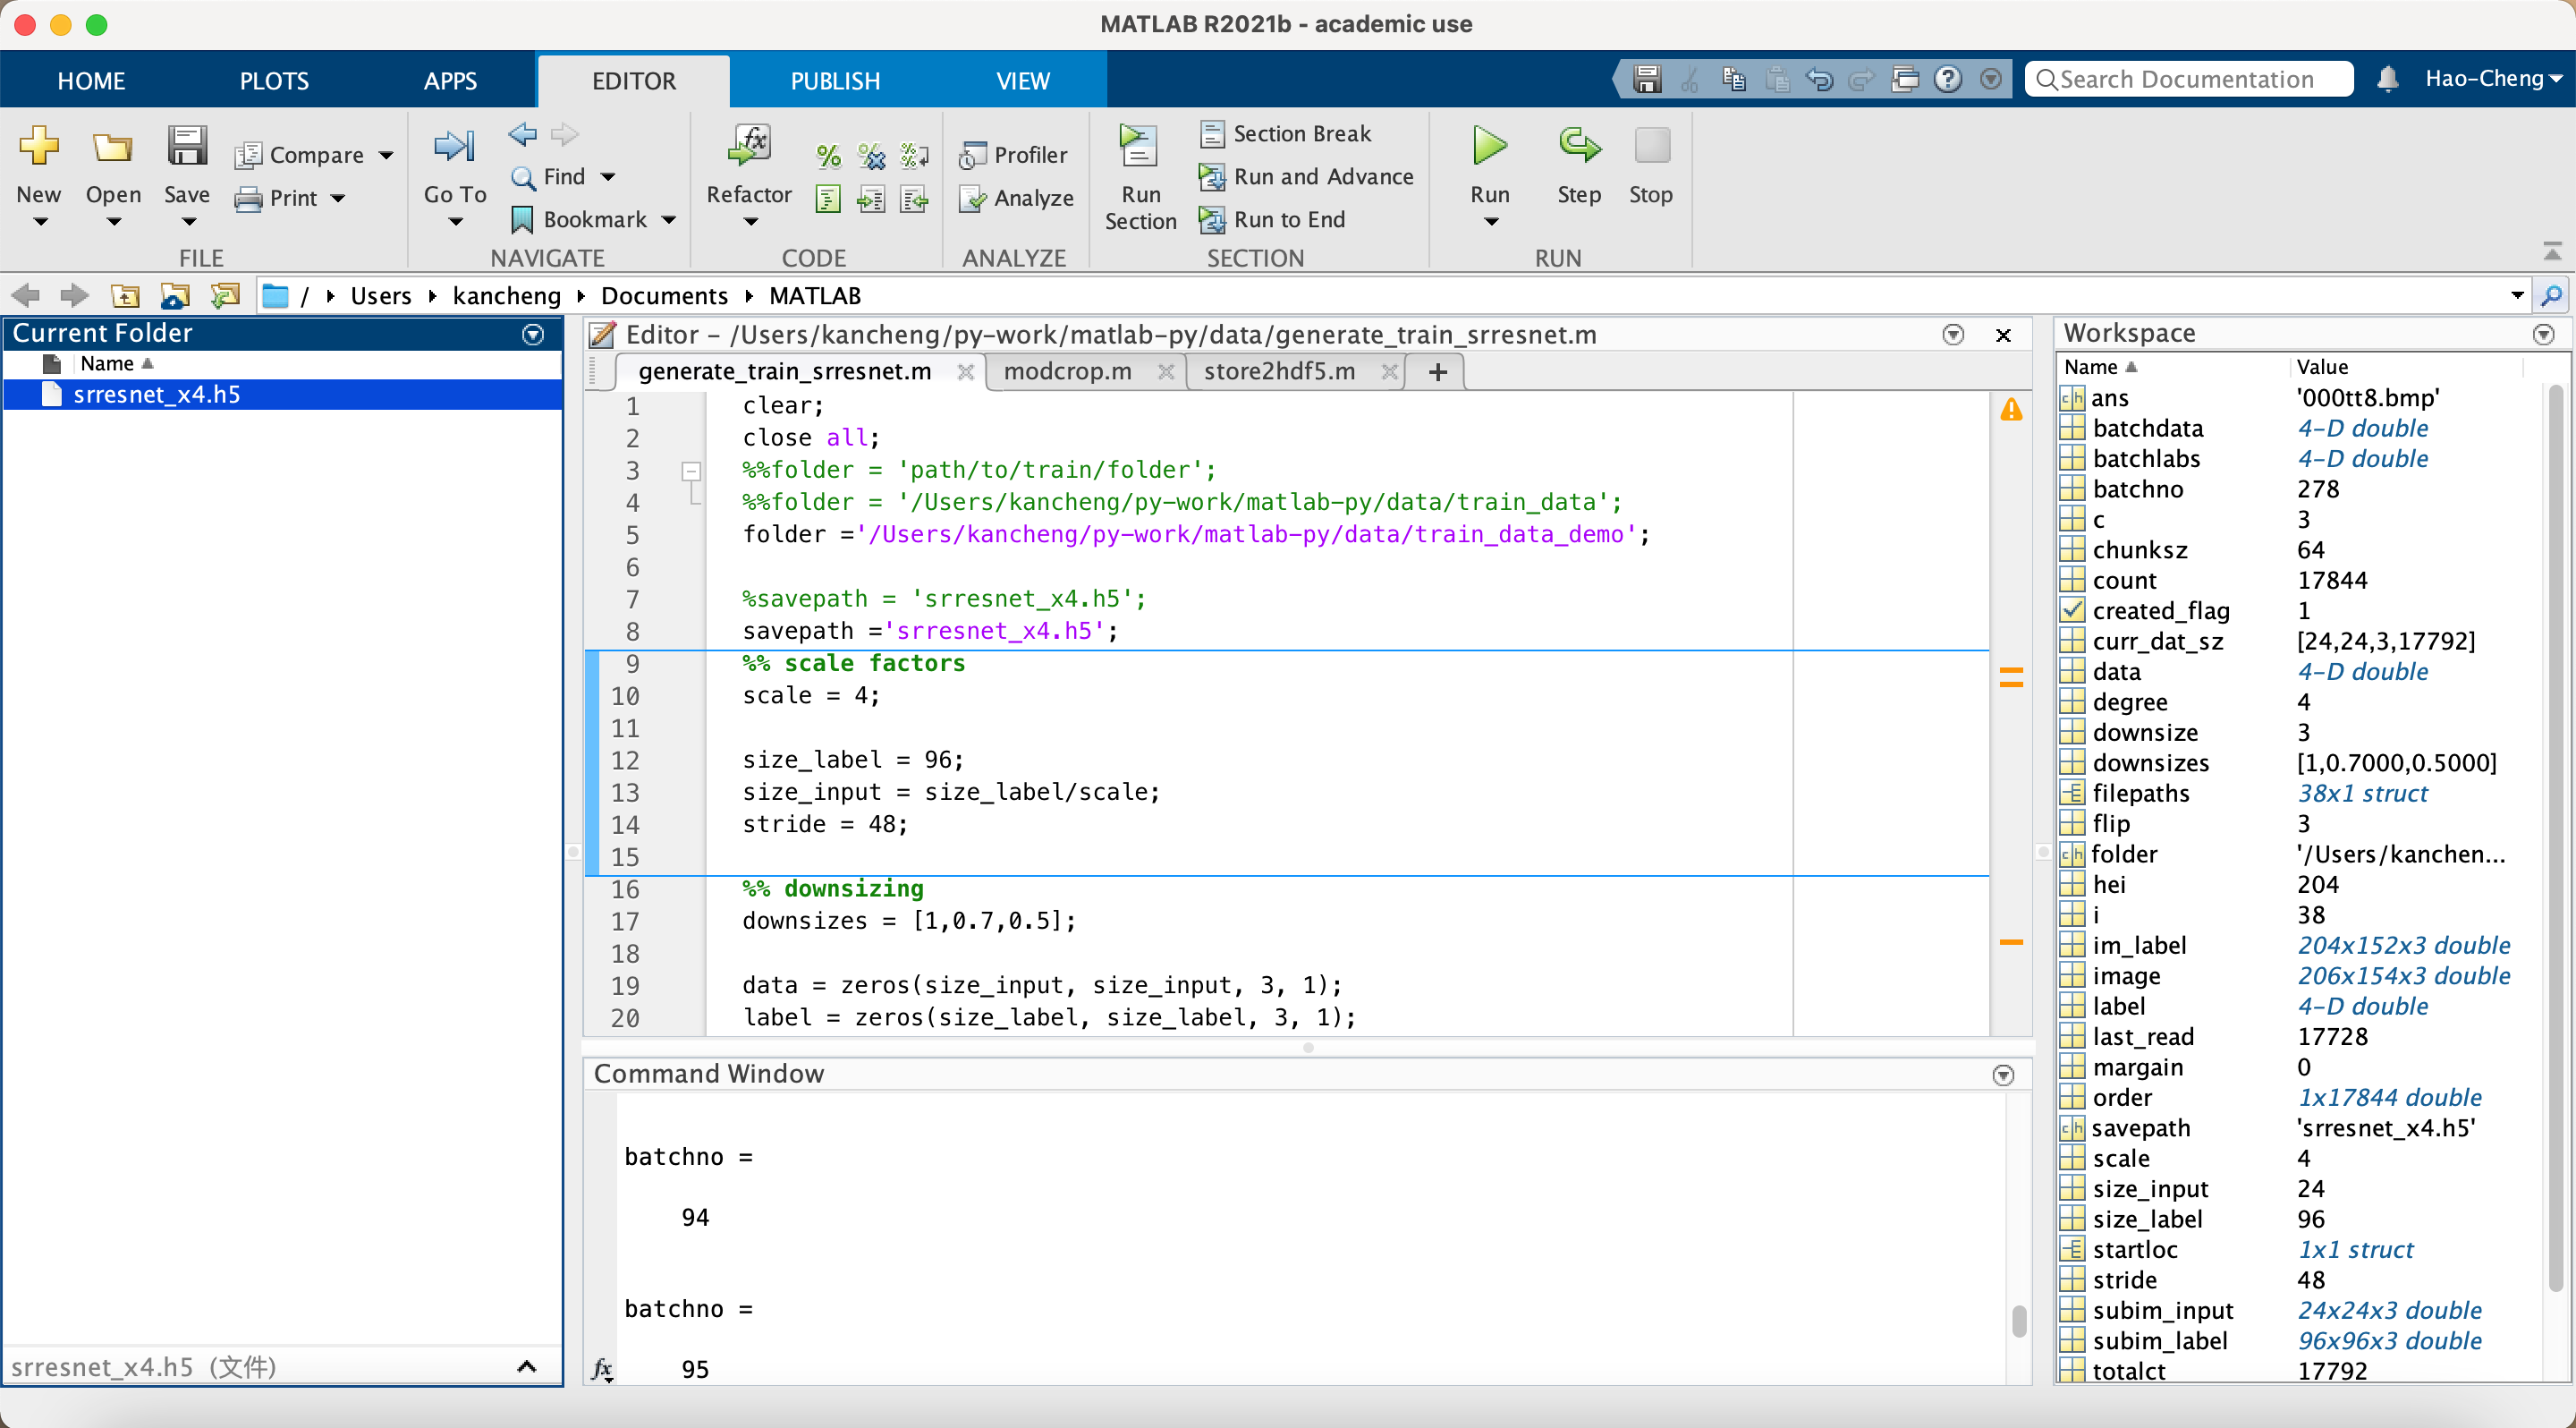
\includegraphics[width=0.9\textwidth]{m1.png} 
\caption{Matlab}
\label{Test}
\end{figure}


% \newpage
\newpage

\section{SR 算法整理}

在此根據 Hongying Liu et al.[1] 將 SR 算法等重要的研究文獻整理,如下所示 : 


\begin{figure}[H]
\centering 
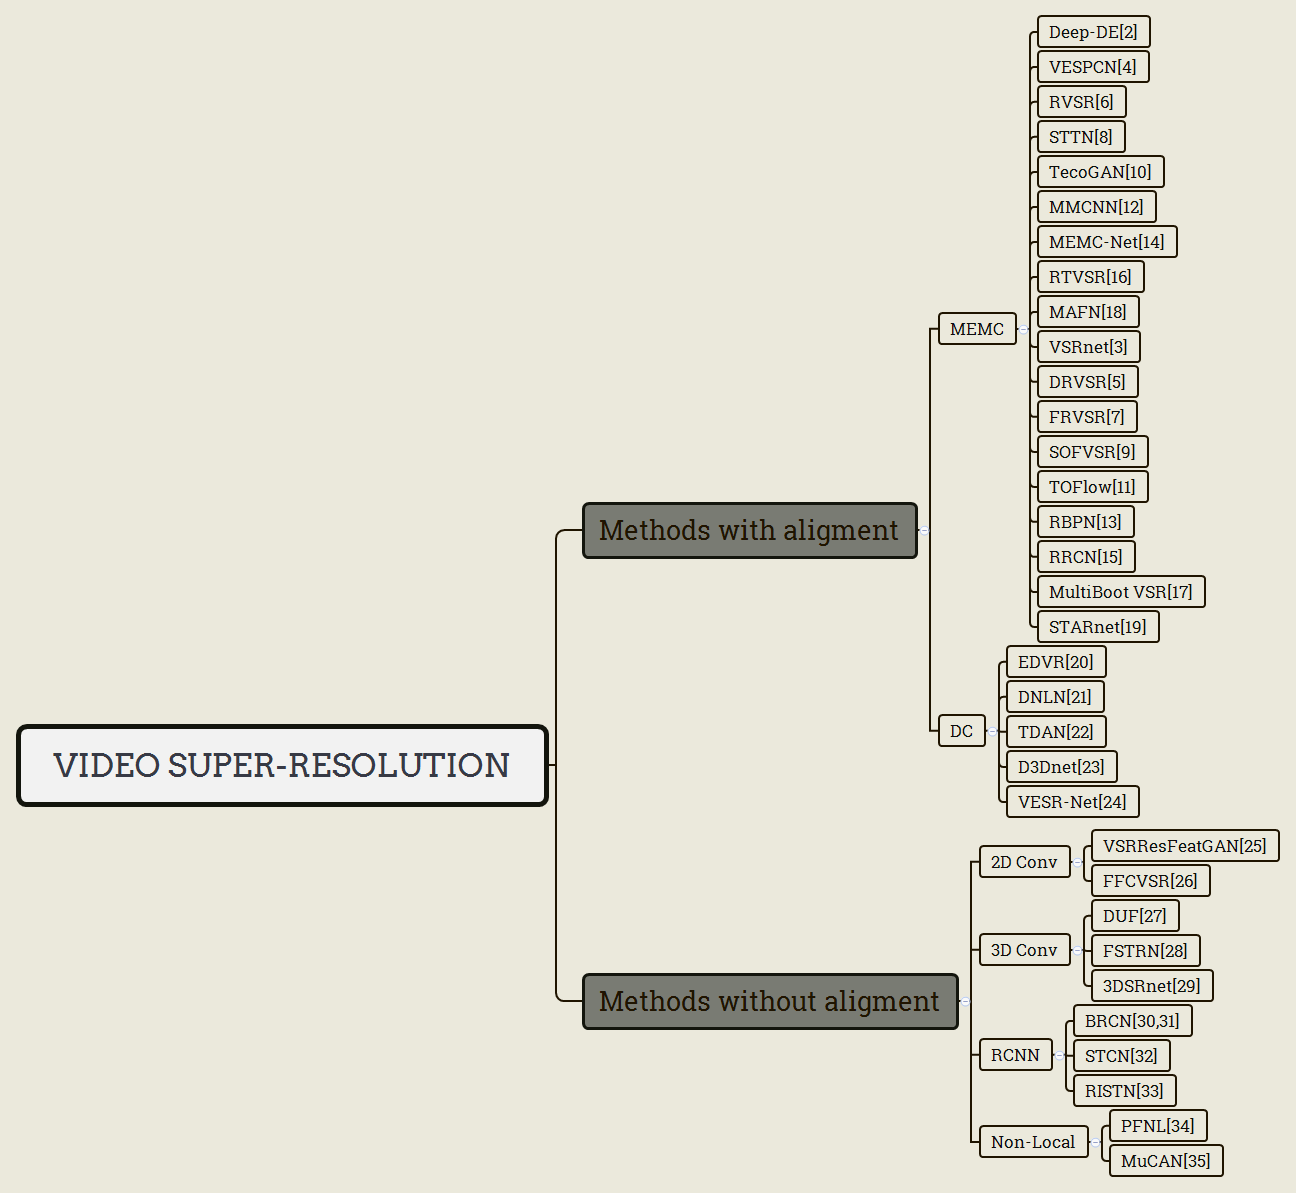
\includegraphics[width=0.9\textwidth]{sr1.png} 
\caption{SR 算法整理}
\label{Test}
\end{figure}

從上面圖中可以看到 MEMC 代表運動估計和補償方法,DC 是可變形卷積方法,3D Conv 是 3D 卷積方法,RCNN 表示基於循環卷積神經網絡的方法。而下表則是近來 SR 算法與分類的整理,而該表也是根據 Hongying Liu et al.[1] 整理而成。



\begin{center}
%\setlength{\tabcolsep}{5mm}{
\resizebox{\textwidth}{80mm}{
\begin{tabular}{cccccc}
\hline
Method & Year & Synonym & Type \\
\hline
Deep-DE [2] & 2015 & Deep Draft-Ensemble Learning & MEMC \\
VSRnet [3] & 2016 & Video Super-Resolution with convolutional neural Networks & MEMC \\
VESPCN [4] & 2017 & Video Efficient Sub-pixel Convolutional Network & MEMC \\
DRVSR [5] & 2017 & Detail-Revealing deep Video Super-Resolution & MEMC \\
RVSR [6] & 2017 & Robust Video Super-Resolution & MEMC \\
FRVSR [7] & 2018 & Frame-Recurrent Video Super-Resolution & MEMC \\
STTN [8] & 2018 & Spatio-Temporal Transformer Network & MEMC \\
SOFVSR [9] & 2018 & Super-resolution Optical Flow for Video SuperResolution & MEMC \\
TecoGAN [10] & 2018 & Temporally coherent GAN & MEMC \\
TOFlow [11] & 2019 & video enhancement with Task-Oriented Flow & MEMC \\
MMCNN [12] & 2019 & Multi-Memory Convolutional Neural Network & MEMC \\
RBPN [13] & 2019 & Recurrent Back-Projection Network & MEMC \\
MEMC-Net [14] & 2019 & Motion Estimation and Motion Compensation Network & MEMC \\
RRCN [15] & 2019 & Residual Recurrent Convolutional Network & MEMC \\
RTVSR [16] & 2019 & Real-Time Video Super-Resolution & MEMC \\
MultiBoot VSR[17] & 2019 & Multi-stage multi-reference Bootstrapping for Video Super-Resolution & MEMC \\
MAFN [18] & 2020 & Motion-Adaptive Feedback Network & MEMC \\
STARnet [19] & 2020 & Space-Time-Aware multi-Resolution network & MEMC \\
EDVR [20] & 2019 & Enhanced Deformable convolutional networks for Video Restoration & DC \\
DNLN [21] & 2019 & Deformable Non-Local Network for Video Super-Resolution & DC \\
TDAN [22] & 2020 & Temporally-Deformable Alignment Network for Video Super-Resolution & DC \\
D3Dnet [23] & 2020 & Deformable 3D Convolution for Video SuperResolution & DC \\
VESR-Net [24] & 2020 & Video Enhancement and Super-Resolution Network & DC \\
VSRResFeatGAN [25] & 2019 & Video Super-Resolution with Residual Networks & 2D Conv \\
FFCVSR [26] & 2019 & Frame and Feature-Context Video SuperResolution & 2D Conv \\
DUF [27] & 2018 & video super-resolution network using Dynamic Upsampling Filters & 3D Conv \\
FSTRN [28] & 2019 & Fast Spatio-Temporal Residual Network for Video Super-Resolution  & 3D Conv \\
3DSRnet [29] & 2019 & 3D Super-Resolution Network & 3D Conv \\
BRCN [30, 31] & 2015/2018 & video super-resolution via Bidirectional Recurrent Convolutional Networks & RCNN \\
STCN [32] & 2017 & Spatio-Temporal Convolutional Network for Video Super-Resolution & RCNN \\
RISTN [33] & 2019 & Residual Invertible Spatio-Temporal Network for Video Super-Resolution & RCNN \\
PFNL [34] & 2019 & Progressive Fusion network via exploiting NonLocal spatio-temporal correlations & Non-Local \\
MuCAN [35] & 2020 & Multi-Correspondence Aggregation Network for Video Super-Resolution & Non-Local \\
\hline
\end{tabular}}
\end{center}

% \newpage
\newpage

\section{參考文獻}

[1] Hongying Liu, Zhubo Ruan, Peng Zhao, Chao Dong, Fanhua Shang, Yuanyuan Liu, Linlin Yang, “Video Super Resolution Based on Deep Learning: A Comprehensive Survey” arXiv preprint arXiv:2007.12928, 2020.

[2] R. Liao, X. Tao, R. Li, Z. Ma, and J. Jia, “Video super-resolution via deep draft-ensemble learning,” in Proc IEEE Int. Conf. Comput. Vis., 2015, pp. 531–539.

[3] A. Kappeler, S. Yoo, Q. Dai, and A. K. Katsaggelos, “Video super-resolution with convolutional neural networks,” IEEE Trans. Comput. Imaging, vol. 2, no. 2, pp. 109–122, June 2016.

[4] J. Caballero, C. Ledig, A. Aitken, A. Acosta, J. Totz, Z. Wang, and W. Shi, “Real-time video superresolution with spatio-temporal networks and motion compensation,” in Proc. IEEE Conf. Comput. Vis. Pattern Recognit., 2017, pp. 2848–2857.

[5] X. Tao, H. Gao, R. Liao, J. Wang, and J. Jia, “Detailrevealing deep video super-resolution,” in Proc IEEE Int. Conf. Comput. Vis., 2017, pp. 4482–4490.

[6] D. Liu, Z. Wang, Y. Fan, X. Liu, Z. Wang, S. Chang, and T. Huang, “Robust video super-resolution with learned temporal dynamics,” in Proc IEEE Int. Conf. Comput. Vis., 2017, pp. 2526–2534.

[7] M. S. M. Sajjadi, R. Vemulapalli, and M. Brown, “Frame-recurrent video super-resolution,” in Proc. IEEE Conf. Comput. Vis. Pattern Recognit., 2018, pp. 6626–6634.

[8] T. H. Kim, M. S. M. Sajjadi, M. Hirsch, and B. Scholkopf, “Spatio-temporal transformer network for video restoration,” in Comput. Vis. - ECCV, 2018, pp. 111–127.

[9] L. Wang, Y. Guo, Z. Lin, X. Deng, and W. An, “Learning for video super-resolution through HR optical flow estimation,” in Proc. Asian Conf. Comput. Vis., 2019, pp. 514–529.

[10] M. Chu, Y. Xie, J. Mayer, L. Leal-Taixe, and N. Thuerey, “Learning Temporal Coherence via Self-Supervision for GAN-based Video Generation,” arXiv e-prints, 2018.

[11] T. Xue, B. Chen, J. Wu, D. Wei, and W. T. Freeman, “Video enhancement with task-oriented flow,” Int. J. Comput. Vis., vol. 127, no. 8, pp. 1106–1125, Aug 2019.

[12] Z. Wang, P. Yi, K. Jiang, J. Jiang, Z. Han, T. Lu, and J. Ma, “Multi-memory convolutional neural network for video super-resolution,” IEEE Trans. Image Process., vol. 28, no. 5, pp. 2530–2544, May 2019.

[13] M. Haris, G. Shakhnarovich, and N. Ukita, “Recurrent back-projection network for video superresolution,” in Proc. IEEE Conf. Comput. Vis. Pattern Recognit., 2019, pp. 3892–3901.

[14] W. Bao, W. Lai, X. Zhang, Z. Gao, and M. Yang, “MEMC-Net: Motion estimation and motion compensation driven neural network for video interpolation and enhancement,” IEEE Trans. Pattern Anal. Mach. Intell., 2019.

[15] D. Li, Y. Liu, and Z. Wang, “Video super-resolution using non-simultaneous fully recurrent convolutional network,” IEEE Trans. Image Process., vol. 28, no. 3, pp. 1342–1355, March 2019.

[16] B. Bare, B. Yan, C. Ma, and K. Li, “Real-time video super-resolution via motion convolution kernel estimation,” Neurocomputing, vol. 367, pp. 236–245, 2019.

[17] R. Kalarot and F. Porikli, “MultiBoot VSR: Multistage multi-reference bootstrapping for video super-resolution,” in Proc. IEEE Conf. Comput. Vis. Pattern Recognit. Workshops, 2019, pp. 2060–2069.

[18] J. Xin, N. Wang, J. Li, X. Gao, and Z. Li, “Video face super-resolution with motion-adaptive feedback cell.” in Proc. AAAI Conf. Artif. Intell., 2020, pp.12 468–12 475.

[19] M. Haris, G. Shakhnarovich, and N. Ukita, “Space-time-aware multi-resolution video enhancement,” in Proc. IEEE/CVF Conf. Comput. Vis. Pattern Recognit., 2020, pp. 2859–2868.

[20] X. Wang, K. C. K. Chan, K. Yu, C. Dong, and C. C. Loy, “EDVR: Video restoration with enhanced deformable convolutional networks,” in Proc. IEEE Conf. Comput. Vis. Pattern Recognit. Workshops, 2019, pp. 1954–1963.

[21] H. Wang, D. Su, C. Liu, L. Jin, X. Sun, and X. Peng, “Deformable non-local network for video super-resolution,” IEEE Access, vol. 7, pp. 177 734–177 744, 2019.

[22] Y. Tian, Y. Zhang, Y. Fu, and C. Xu, “TDAN: Temporally-deformable alignment network for video super-resolution,” in Proc. IEEE Conf. Comput. Vis. Pattern Recognit., 2020, pp. 3360–3369.

[23] X. Ying, L. Wang, Y. Wang, W. Sheng, W. An, and Y. Guo, “Deformable 3d convolution for video super-resolution,” arXiv preprint arXiv:2004.02803, 2020.

[24] J. Chen, X. Tan, C. Shan, S. Liu, and Z. Chen, “Vesrnet: The winning solution to youku video enhancement and super-resolution challenge,” arXiv preprint arXiv:2003.02115, 2020.

[25] A. Lucas, S. LApez-Tapia, R. Molina, and A. K. Katsaggelos, “Generative adversarial networks and perceptual losses for video super-resolution,” IEEE Trans. Image Process., vol. 28, no. 7, pp. 3312–3327, July 2019.

[26] B. Yan, C. Lin, and W. Tan, “Frame and featurecontext video super-resolution,” in Proc. AAAI Conf. Artif. Intell., 2019, pp. 5597–5604.

[27] Y. Jo, S. W. Oh, J. Kang, and S. J. Kim, “Deep video super-resolution network using dynamic upsampling filters without explicit motion compensation,” in Proc. IEEE Conf. Comput. Vis. Pattern Recognit., 2018, pp. 3224–3232.

[28] S. Li, F. He, B. Du, L. Zhang, Y. Xu, and D. Tao, “Fast spatio-temporal residual network for video super-resolution,” in Proc. IEEE Conf. Comput. Vis. Pattern Recognit., 2019, pp. 10 522–10 531.

[29] S. Y. Kim, J. Lim, T. Na, and M. Kim, “Video superresolution based on 3d-cnns with consideration of scene change,” in Proc. IEEE Int. Conf. Image Process., 2019, pp. 2831–2835.

[30] Y. Huang, W. Wang, and L. Wang, “Bidirectional recurrent convolutional networks for multi-frame super-resolution,” in Advances in Neural Information Processing Systems, 2015, pp. 235–243.

[31] Y. Huang, W. Wang, and L. Wang, “Video superresolution via bidirectional recurrent convolutional networks,” IEEE Trans. Pattern Anal. Mach. Intell., vol. 40, no. 4, pp. 1015–1028, April 2018.

[32] J. Guo and H. Chao, “Building an end-to-end spatial-temporal convolutional network for video super-resolution,” in Proc. AAAI Conf. Artif. Intell., 2017, pp. 4053–4060.

[33] X. Zhu, Z. Li, X. Zhang, C. Li, Y. Liu, and Z. Xue, “Residual invertible spatio-temporal network for video super-resolution,” in Proc. AAAI Conf. Artif. Intell., 2019, pp. 5981–5988.

[34] P. Yi, Z. Wang, K. Jiang, J. Jiang, and J. Ma, “Progressive fusion video super-resolution network via exploiting non-local spatio-temporal correlations,”in Proc IEEE Int. Conf. Comput. Vis., 2019, pp. 3106–3115.

[35] W. Li, X. Tao, T. Guo, L. Qi, J. Lu, and J. Jia,“Mucan: Multi-correspondence aggregation network for video super-resolution,” arXiv preprint arXiv:2007.11803, 2020.


%\begin{enumerate}
%\item Y
%\item A
%\end{enumerate}

% \newpage

\clearpage

\end{document}